
\chapter{永磁同步电机数学模型}\label{ch:model}
\section{引言}
本章主要介绍永磁同步电机的数学模型。永磁同步电机的数学模型是矢量控制的重要基础。本章先介绍了永磁同步电机结构特点,然后介绍了在不同坐标系下的电机动态方程,为矢量后续章节的矢量控制打下基础。

\section{永磁同步电机建模}
根据永磁同步电机转子永磁体安装方式的不同,可将永磁同步电机分为表面贴磁型和内嵌永磁体型。如图\ref{fig:motorType}所示,(a)为表面贴磁型永磁同步电机,永磁体固定在转子表面。(b)为内嵌永磁体型永磁同步电机,永磁体安装在转子铁心内部。两种不同的结构对于电机磁路有不同的影响。在表面贴磁型永磁同步电机中,理想情况下,d轴和q轴磁路磁阻相同,电感相等。而对于内嵌永磁体型永磁同步电机来说,由于q轴磁路磁阻小于d轴磁路磁阻,所以q轴电感大于d轴电感。
\begin{figure}[H]
	\centering
	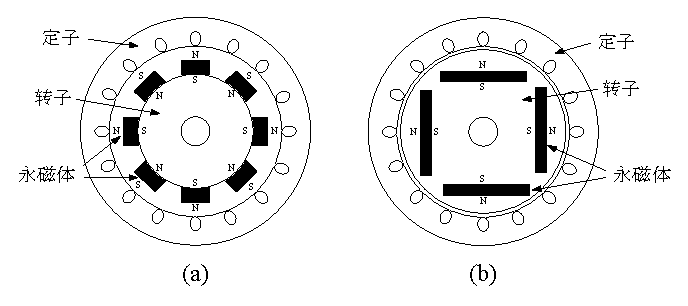
\includegraphics[width=0.7\textwidth]{figs/motor-types.eps}
	\caption{不同转子类型的永磁同步电机.(a)表面贴磁型(b)内嵌永磁体型}
	\label{fig:motorType}
\end{figure}
图\ref{fig:PMSM}所示为一对极表面贴磁型永磁同步电机简化示意图,图中定子三相绕组用分别用$AA-$,$BB-$,$CC-$三个线圈表示,线圈上的叉和点分别表示电流入和流出纸面。三相绕组空间相隔120度电角度,其磁轴用a,b,c表示。图中$\theta_{r}$表示转子北极与定子磁轴a的夹角,也就是转子位置电角度。
\begin{figure}[H]
	\centering
	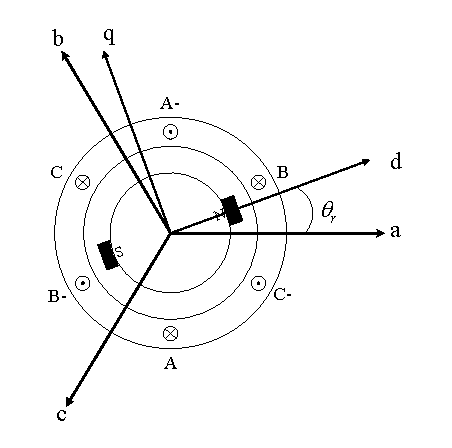
\includegraphics[width=0.6\textwidth]{figs/PMSM.eps}
	\caption{表面贴磁型永磁同步电机示意图}
	\label{fig:PMSM}
\end{figure}
\section{abc坐标定子电压方程}
三相永磁同步电机在静止abc参考系下的定子电压方程可以表示为:
\begin{equation}\label{eq:voltage}
\begin{bmatrix}v_{a}\\v_{b}\\v_{c} \end{bmatrix}
=
\begin{bmatrix}R&0&0\\0&R&0\\0&0&R\end{bmatrix}
\begin{bmatrix} i_{a}\\i_{b}\\i_{c}\end{bmatrix}
+
\frac d{dt} \begin{bmatrix}\lambda_{a}\\\lambda_{b}\\\lambda_{c}\end{bmatrix}
\end{equation} 
\ref{eq:voltage}中$v_{a},v_{b},v_{c}$分别表示定子三相电压,R代表定子电阻,$\lambda_{a},\lambda_{b},\lambda_{c}$代表三相绕组磁链。永磁同步电机中三相绕组磁链可以表示为:
\begin{equation}
\begin{bmatrix}\label{eq:flux}
\lambda_{a}\\\lambda_{b}\\\lambda_{c}\end{bmatrix}=\begin{bmatrix}
L_{aa}&M_{ab}&M_{ac}\\M_{ab}&L_{bb}&M_{bc}\\M_{ac}&M_{bc}&L_{cc}
\end{bmatrix}
\begin{bmatrix}
i_{a}\\i_{b}\\i_{c}
\end{bmatrix}
+\begin{bmatrix}\lambda_{pm,a}\\\lambda_{pm,b}\\\lambda_{pm,c}\end{bmatrix}
\end{equation}
其中$L_{aa}$,$L_{bb}$,$L_{cc}$分别表示定子三相绕组自感,$M_{ab}$,$M_{ac}$,$M_{bc}$分别表示ab,ac,bc两相绕组互感,转子永磁体在三相绕组产生的磁链为转子电角度$\theta_{r}$的函数:
\begin{equation}\label{eq:flux1}
\begin{bmatrix}\lambda_{pm,a}\\\lambda_{pm,b}\\\lambda_{pm,c}\end{bmatrix}
=
\lambda_{mpm}\begin{bmatrix}\cos(\theta_{r})\\\cos(\theta_{r}-120^{o})\\\cos(\theta_{r}+120^{o})\end{bmatrix} 
\end{equation}
将公式\ref{eq:flux}和\ref{eq:flux1}组合在一起,可以得到定子磁链方程为:
\begin{equation}\label{eq:flux2}
\begin{bmatrix}
\lambda_{a}\\\lambda_{b}\\\lambda_{c}
\end{bmatrix}
=
\begin{bmatrix}
L_{aa}&M_{ab}&M_{ac}\\M_{ab}&L_{bb}&M_{bc}\\M_{ac}&M_{bc}&L_{cc}
\end{bmatrix}
\begin{bmatrix}
i_{a}\\i_{b}\\i_{c}
\end{bmatrix}
+
\lambda_{mpm}\begin{bmatrix}\cos(\theta_{r})\\\cos(\theta_{r}-120^{o})\\\cos(\theta_{r}+120^{o})\end{bmatrix}
\end{equation}
其中,$\lambda_{mpm}$为转子永磁体在定子上产生相磁链的最大值。由于电机转子位置不同影响电机磁路结构,电机电感参数随着转子位置的改变而改变,这些参数计算是电机建模的重要部分,传统方法采用对空间磁密积分的方法\cite{krause2013analysis}求电感参数,较为繁琐。文献\cite{lu2011simple}提出了一种基于矢量投影的求取电机中电感参数的方法,可以比较方便的计算电感参数。
式\ref{eq:flux}中三相绕组自感参数可以表示为:
\begin{align}
L_{aa}&= L_{\sigma}+L_{A}-L_{B}\cos(2\theta_{r})\label{eq:Laa}\\
L_{bb}&= L_{\sigma}+L_{A}-L_{B}\cos[2(\theta_{r}-120^{o})]\label{eq:Lbb}\\ 
L_{cc}&= L_{\sigma}+L_{A}-L_{B}\cos[2(\theta_{r}+120^{o})]\label{eq:Lcc}
\end{align}
其中$L_{\sigma}$定子绕组漏电感,$L_{A}$和$L_{B}$定义为:
\begin{align}\label{eq:induc2}
L_{A}= \frac{L_{aad}+L_{aaq}}{2}\\
L_{B}= \frac{L_{aad}-L_{aaq}}{2} 
\end{align}
其中$L_{aad}$为当转子位置$\theta_{r}=0$时定子a相自感,$L_{aaq}$为当转子位置$\theta_{r}=90^{o}$时定子a相自感。
此时,定子三相绕组之间的互感可以表示为:
\begin{align}
M_{ab}&=-\frac{1}{2}L_{A}-L_{B}\cos2(\theta_{r}-60^{o})\label{eq:Mab}\\
M_{ac}&=-\frac{1}{2}L_{A}-L_{B}\cos2(\theta_{r}+60^{o})\label{eq:Mac}\\
M_{bc}&=-\frac{1}{2}L_{A}-L_{B}\cos2(\theta_{r})\label{eq:Mbc}
\end{align}
上结果可以看出,静止abc参考下的数学模型由于电机电感参数随着转子位置的改变十分复杂,不利于分析。
\section{$\alpha\beta$坐标电机模型}\label{sec:model}
为了方便分析,通常采用坐标变换的方法简化电机数学模型,坐标变换的实质在于变量代换,通过变量代换降低描述电机微分方程的复杂度\cite{reference_frame}。常用的坐标变换为$\alpha\beta$变换和$dq$变换。
\subsection{$\alpha\beta$变换}
$\alpha\beta$变换是将三相坐标的量等效为两相静止坐标上。将三相电压看成一个空间矢量,其三个分量分别在abc轴上,abc互隔$120^{o}$。该空间矢量可以在一个垂直坐标系中表示。如图\ref{fig:alphabeta}所示,$\alpha$轴与a轴重合,$\beta$轴与$\alpha$垂直。
\begin{figure}[H]
	\centering
	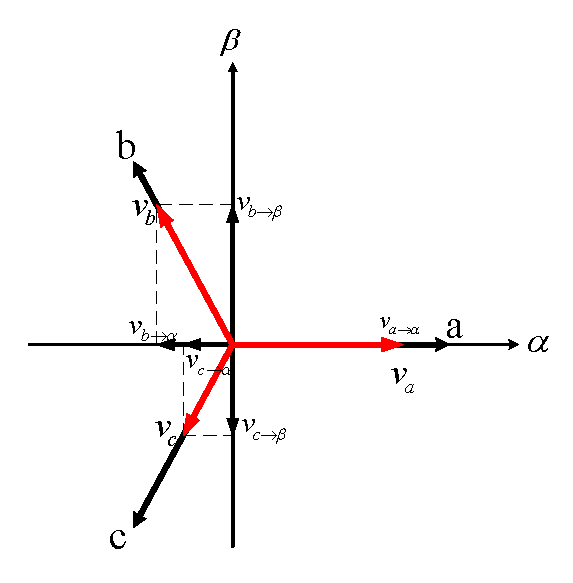
\includegraphics[width=0.7\textwidth]{figs/alphabeta.eps}
	\caption{静止abc坐标到$\alpha\beta$坐标变换}
	\label{fig:alphabeta}
\end{figure}
将电压矢量投影到$\alpha\beta$轴可以得到abc坐标到$\alpha\beta$坐标的变换矩阵:
\begin{equation}\label{eq:abc2ab}
T=\frac{2}{3}\begin{bmatrix}1&-\frac{1}{2}&-\frac{1}{2}\\0&\frac{\sqrt{3}}{2}&-\frac{\sqrt{3}}{2}\end{bmatrix}
\end{equation}
同样,将$\alpha\beta$轴的量投影在$abc$参考下可以得到$\alpha\beta$到$abc$的变换矩阵:
\begin{equation}
T^{-1} =\frac32\begin{bmatrix} \frac23 & 0 \\
-\frac{1}{3} & \frac{\sqrt{3}}{3} \\
-\frac{1}{3} & -\frac{\sqrt{3}}{3} \end{bmatrix} 
\end{equation}
严格地讲,矩阵$T$不是方阵,不存在逆。此处$T^{-1}$为$\alpha\beta$到$abc$的变换矩阵,而不是$T$的逆矩阵。
\subsection{$\alpha\beta$坐标下定子电压方程}
将方程\ref{eq:voltage}两边同时乘以变换矩阵$T$可以得到:
\begin{equation}\label{eq:vab}
\begin{bmatrix}
v_{\alpha}\\v_{\beta}
\end{bmatrix}
=
\begin{bmatrix}
R&0\\0&R
\end{bmatrix}
\begin{bmatrix}
i_{\alpha}\\i_{\beta}
\end{bmatrix}
+
\frac{d}{dt}\begin{bmatrix}
\lambda_{\alpha}\\\lambda_{\beta}
\end{bmatrix}
\end{equation}
其中
\begin{equation}\label{eq:fab}
\begin{bmatrix}
\lambda_{\alpha}\\\lambda_{\beta}
\end{bmatrix}
=T\begin{bmatrix}
L_{aa}&M_{ab}&M_{ac}\\M_{ab}&L_{bb}&M_{bc}\\M_{ac}&M_{bc}&L_{cc}\end{bmatrix}T^{-1}\begin{bmatrix}
i_{\alpha}\\i_{\beta}
\end{bmatrix}
+
\lambda_{mpm}T\begin{bmatrix}\cos(\theta_{r})\\\cos(\theta_{r}-120^{o})\\\cos(\theta_{r}+120^{o})\end{bmatrix}
\end{equation}
将自感参数\ref{eq:Laa}-\ref{eq:Lcc}和互感参数\ref{eq:Mab}-\ref{eq:Mbc}代入入$\alpha\beta$轴磁链方程\ref{eq:fab}中可以求得:
\begin{align}\label{eq:fab1}
\begin{bmatrix}
\lambda_{\alpha}\\\lambda_{\beta}
\end{bmatrix}
&=
\begin{bmatrix}
L_{\sigma}&0\\0&L_{\sigma}
\end{bmatrix}
\begin{bmatrix}
i_{\alpha}\\i_{\beta}
\end{bmatrix}
+
\frac{3}{2}\begin{bmatrix}
L_{A}-L_{B}\cos(2\theta_{r})&L_{B}\sin(2\theta_{r})\\-L_{B}\sin(2\theta_{r})&L_{A}+L_{B}\cos(2\theta_{r})
\end{bmatrix}\begin{bmatrix}
i_{\alpha}\\i_{\beta}
\end{bmatrix}\nonumber\\&+
\lambda_{mpm}\begin{bmatrix}
\cos(\theta_{r})\\\sin(\theta_{r})
\end{bmatrix}
\end{align}
可以看到用$\alpha\beta$表达的电机数学模型,将abc三相的量,用$\alpha\beta$两相表示出来,简化了方程表达。但是,磁链方程中电感参数矩阵依然随着转子位置的改变而发生改变,因此需要进一步将$\alpha\beta$变换成为旋转坐标系,进一步简化。
\section{dq坐标电机模型}
\subsection{$\alpha\beta$到dq变换}
如图\ref{fig:dq}所示,为$\alpha\beta$坐标和旋转dq坐标系。其中d轴与$\alpha$轴夹角为转子位置电角度。
\begin{figure}[H]
	\centering
	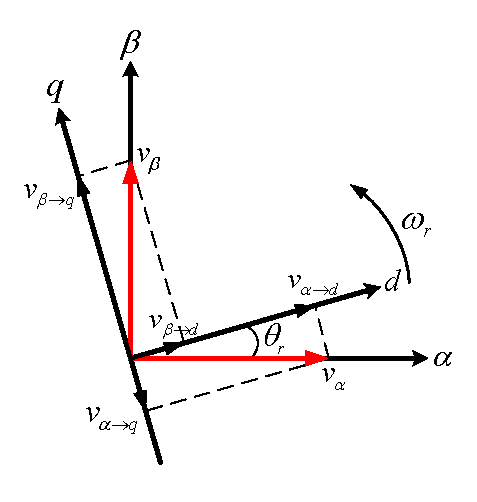
\includegraphics[width=0.6\textwidth]{figs/dq.eps}
	\caption{表面贴磁型永磁同步电机示意图}
	\label{fig:dq}
\end{figure}
根据矢量投影的方法,可以推导出$\alpha\beta$到$dq$变换的矩阵为:
\begin{equation}\label{eq:dq}
K=\begin{bmatrix}\cos(\theta_{r})&\sin(\theta_{r})\\
-\sin(\theta_{r})&\cos(\theta_{r})
\end{bmatrix}
\end{equation}
反过来,dq到$\alpha\beta$变换矩阵可以推导为:
\begin{equation}\label{eq:inversedq}
K^{-1}=\begin{bmatrix}\cos(\theta_{r})&-\sin(\theta_{r})\\\sin(\theta_{r})&\cos(\theta_{r})
\end{bmatrix}
\end{equation}
\section{dq坐标电压方程}
将方程$\alpha\beta$坐标下的电压方程\ref{eq:vab}两边同时乘以$\alpha\beta$到dq变换矩阵K有:
\begin{align}\label{eq:vdq}
\begin{bmatrix}
v_{d}\\v_{q}
\end{bmatrix}
&=
\begin{bmatrix}
R&0\\0&R
\end{bmatrix}
\begin{bmatrix}
i_{d}\\i_{q}
\end{bmatrix}
+
K\frac{d}{dt}\left[K^{-1}\begin{bmatrix}
\lambda_{d}\\\lambda_{q}\end{bmatrix}\right]\nonumber\\
&=\begin{bmatrix}
R&0\\0&R
\end{bmatrix}
\begin{bmatrix}
i_{d}\\i_{q}\end{bmatrix}+K\frac{d}{dt}\left(K^{-1}\right)\begin{bmatrix}
\lambda_{d}\\\lambda_{q}\end{bmatrix}+\frac{d}{dt}\begin{bmatrix}\lambda_{d}\\\lambda_{q}\end{bmatrix}
\end{align}
其中,
\begin{align}\label{eq:trans}
K\frac{d}{dt}\left(K^{-1}\right)&=K\frac{d}{d\theta_{r}}\left(K^{-1}\right)\frac{d}{dt}\left(\theta_{r}\right)\nonumber\\
&=\omega_{r}\begin{bmatrix}0&-1\\1&0\end{bmatrix}
\end{align}
所以dq坐标下的电压方程可以表达为:
\begin{align}\label{eq:vdq_final}
\begin{bmatrix}
v_{d}\\v_{q}
\end{bmatrix}
=
\begin{bmatrix}
	R&0\\0&R
\end{bmatrix}
\begin{bmatrix}
	i_{d}\\i_{q}\end{bmatrix}
	+
	\omega_{r}\begin{bmatrix}0&-1\\1&0\end{bmatrix}
	\begin{bmatrix}
	\lambda_{d}\\\lambda_{q}\end{bmatrix}
	+
	\frac{d}{dt}\begin{bmatrix}\lambda_{d}\\\lambda_{q}\end{bmatrix}
\end{align}
将$\alpha\beta$坐标下的磁链方程\ref{eq:fab1}两端同时乘以$\alpha\beta$到dq变换矩阵K有:
\begin{align}
\begin{bmatrix}
\lambda_{d}\\\lambda_{q}
\end{bmatrix}&=
\frac{3}{2}K\begin{bmatrix}
L_{A}-L_{B}\cos(2\theta_{r})&L_{B}\sin(2\theta_{r})\\-L_{B}\sin(2\theta_{r})&L_{A}+L_{B}\cos(2\theta_{r})
\end{bmatrix}K^{-1}\begin{bmatrix}i_{d}\\i_{q}
\end{bmatrix}\nonumber\\&
+\begin{bmatrix}
L_{\sigma}&0\\0&L_{\sigma}
\end{bmatrix}
\begin{bmatrix}
i_{d}\\i_{q}
\end{bmatrix}+
\lambda_{mpm}\begin{bmatrix}
1\\0
\end{bmatrix}
\end{align}
将电感定义方程\ref{eq:induc2},矩阵变换方程\ref{eq:dq}和反变换方程\ref{eq:inversedq}带入上式中化简可得到:
\begin{align}\label{eq:calculation}
\frac{3}{2}K\begin{bmatrix}
L_{A}-L_{B}\cos(2\theta_{r})&L_{B}\sin(2\theta_{r})\\-L_{B}\sin(2\theta_{r})&L_{A}+L_{B}\cos(2\theta_{r})\end{bmatrix}K^{-1}&=
\frac{3}{2}\begin{bmatrix}L_{aad}\\L_{aaq}\end{bmatrix}
\end{align}
所以,dq磁链方程为:
\begin{align}\label{eq:fluxdq}
\begin{bmatrix}
\lambda_{d}\\\lambda_{q}
\end{bmatrix}
&=\begin{bmatrix}
L_{\sigma}&0\\0&L_{\sigma}\end{bmatrix}
\begin{bmatrix}
i_{d}\\i_{q}
\end{bmatrix}
+\frac{3}{2}\begin{bmatrix}
L_{aad}&0\\0&L_{aaq}\end{bmatrix}
\begin{bmatrix}
i_{d}\\i_{q}
\end{bmatrix}
+
\lambda_{mpm}\begin{bmatrix}
1\\0
\end{bmatrix}\nonumber\\
&
\end{align}
其中$L_{d}$和$L_{q}$定义为:
\begin{align}
L_{d}=L_{\sigma}+\frac{3}{2}L_{aad}\\
L_{q}=L_{\sigma}+\frac{3}{2}L_{aaq}
\end{align}
所以dq轴磁链方程可以表达为:
\begin{align}\label{eq:fluxdq_final}
\begin{bmatrix}
\lambda_{d}\\\lambda_{q}
\end{bmatrix}
=\begin{bmatrix}
	L_{d}&0\\0&L_{q}
\end{bmatrix}\begin{bmatrix}
	i_{d}\\i_{q}
\end{bmatrix}
+
\lambda_{mpm}\begin{bmatrix}
	1\\0
\end{bmatrix}
\end{align}
可以看到,在dq坐标系中,永磁同步电机的电压方程,磁链方程形式比较简单。d轴电感和q轴电感为常数,这是因为,在dq坐标系中,dq轴与转子相对静止,dq轴磁路固定而不受转子位置的影响。
\section{电磁转矩方程}
本节主要介绍dq坐标下的电磁转矩方程,利用功率守恒的方法导出dq坐标下的电磁转矩表达式。
永磁同步电机运行时,输入电机的瞬时功率按照abc坐标变量可以表达为:
\begin{align}
p = v_{a}i_{a}+v_{b}i_{b}+v_{c}i_{c}
\end{align}
变换到dq坐标系表达式为:
\begin{equation}\label{eq:dqpower}
p = \frac{3}{2}(v_{d}i_{d}+v_{q}i_{q})
\end{equation}
将$v_{d}$和$v_{q}$按照\ref{eq:vdq_final}所述,代入\ref{eq:dqpower}中有:
\begin{align}
p&=\frac{3}{2}(Ri_{d}^2+Ri_{q}^2)+\frac{3}{2}(L_{d}i_{d}\frac{d}{dt}i_{d}+L_{q}i_{q}\frac{d}{dt}i_{q})\nonumber\\
&+\frac{3}{2}\left[\omega_{r}\left(\lambda_{mpm}i_{q}+(L_{d}-L_{q})i_{d}i_{q}\right)\right]
\end{align}
其中$\frac{3}{2}\left[\omega_{r}\left(\lambda_{mpm}i_{q}+(L_{d}-L_{q})i_{d}i_{q}\right)\right]$表示电机输出的功率,而电机输出的机械功率为电磁转矩与机械转速的乘积,即:
\begin{equation}
p_{e}=T_{e}\frac{\omega_{r}}{P}
\end{equation}
其中P为电机极对数。
所以电磁转矩表示式为:
\begin{align}
T_{e}=\frac{3}{2}P\left[\left(\lambda_{mpm}i_{q}+(L_{d}-L_{q})i_{d}i_{q}\right)\right]
\end{align}
对于表面贴磁型永磁同步电机来讲,d轴电感和q轴电感相等,因此转矩表达式可以进一步简化为:
\begin{align}
T_{e}=\frac{3}{2}P\lambda_{mpm}i_{q}
\end{align}
\section{运动平衡方程}
永磁同步电机系统运动平衡方程\ref{eq:mechanical}描述电磁转矩和转速的关系,其中$J_{m}$为系统转动惯量,$B_{m}$为摩擦系数,$T_{L}$为电机负载转矩。
\begin{equation}\label{eq:mechanical}
T_{e}-T_{L}=J_{m}\frac{d\omega_{m}}{dt}+B_{m}\omega_{m} 
\end{equation}
其中机械转速为
\begin{equation}
\omega_{m} = \frac{\omega_{r}}{P}
\end{equation}
\section{本章小结}
永磁同步电机dq动态数学模型为矢量控制的重要基础内容,本章主要介绍了永磁同步电机的结构特点,详细导出了永磁同步电机不同坐标系下的电压、磁链方程、和运动平衡方程为后续矢量控制章节打下坚实基础。